%Considerando ahora además los 5 matches siguientes
%(por lo tanto, 6 secuencias encontradas) que sean en especies distintas
%(de modo que si hay más de uno en la misma especie, se ignoran las "repeticiones"),
%
%    * ¿En qué organismos están?
%		¿Son especies cercanas a las del primer match?
\subsection{Organismos}

\begin{enumerate}
	\item \emph{hypothetical protein LOAG\_10175} $[$Loa loa$]$~\cite{match2}
	\begin{itemize}
		\item Familia:

			Eukaryota; Metazoa; Nematoda; Chromadorea; Spirurida; Filarioidea;Onchocercidae; Loa.
		\item Hypothetical Protein:

			Es una proteína en que su experiencia ha sido predicha pero existen evidencias experimentales de que se expresa en vivo.
		\item Loa Loa:

			Gusano nemátodo (vulgarmente llamado gusanos redondos) y parásito de África central y occidental, son transmitidos a través de los tábanos, causa filariasis.
		\item Imagen:

			\begin{figure}[!h]
				  \subfigure[Microfilaria de Loa Loa]
				  {
				    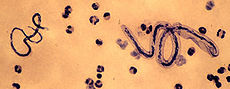
\includegraphics[width=0.32\linewidth, height=!]{img/2-1}
				    \label{fig:match2-1}
				  }
				  \subfigure[Loa Loa dentro del ojo]
				  {
				    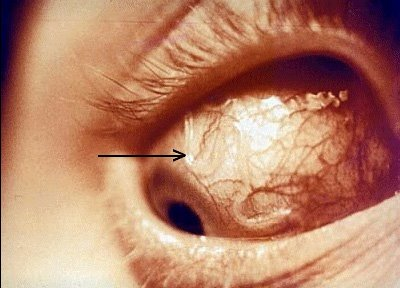
\includegraphics[width=0.32\linewidth, height=!]{img/2-2}
				    \label{fig:match2-2}
				  }
				  \subfigure[Loa Loa fuera del ojo]
				  {
				    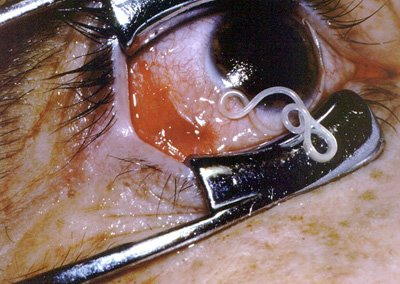
\includegraphics[width=0.32\linewidth, height=!]{img/2-3}
				    \label{fig:match2-3}
				  }
				  \label{fig:match2}
				  \caption{hypothetical protein LOAG\_10175 $[$Loa loa$]$}
		\end{figure}
	\end{itemize}


	\item \emph{Tryptophanase} $[$Rhodobacter sp. SW2$]$~\cite{match3}
	\begin{itemize}
		\item Familia:
			
			Bacteria; Proteobacteria; Alphaproteobacteria; Rhodobacterales;Rhodobacteraceae; Rhodobacter.
		\item Tryptophanase:

			Esta triptofanasa es una enzima catalizadora básicamente reacciones de conversión de triptofano
			a indol.
			El indol se produce naturalmente en la heces fecales humanas produciendo un intenso olor,
			sin embargo en muy bajas concentraciones tiene aroma floral.
		\item Rhodobacter sp. SW2:
			Se encuentra en las rhodobacter, que son microorganismos fotosisnteticos los cuales
			se establecen en aguas dulces y entornos marinos.
		\item Imagen\\
			\begin{figure}[!h]
			\begin{center}
				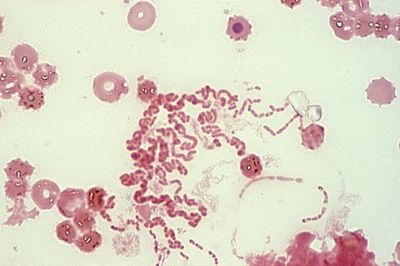
\includegraphics[width=0.32\linewidth, height=!]{img/3}
				\caption{Rhodobacter capsulatus Hemoc}
			    \label{fig:match3}
			\end{center}
			\end{figure}
	\end{itemize}


	\item \emph{hypothetical protein Bm1\_46260} $[$Brugia malayi$]$~\cite{match4}
	\begin{itemize}
		\item Familia:

			Eukaryota; Metazoa; Nematoda; Chromadorea; Spirurida; Filarioidea;Onchocercidae; Brugia.
		\item hypothetical protein Bm1\_46260:

			Es una proteína en que su experiencia ha sido predicha pero existen evidencias experimentales
			de que se expresa en vivo.
		\item Brugia malayi:
			
			Nemátodo espirúrido, son transmitidos por mosquitos, causa en el hombre filariasis.
		\item Imagen
			\begin{figure}[!h]
			\begin{center}
				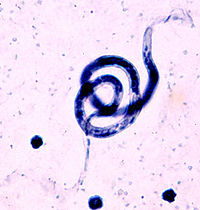
\includegraphics[width=0.32\linewidth, height=!]{img/4}
				\caption{Brugia malayi}
			    \label{fig:match4}
			\end{center}
			\end{figure}
	\end{itemize}

	\item \emph{hypothetical protein PD0579} $[$Xylella fastidiosa Temecula1$]$~\cite{match5}
	\begin{itemize}
		\item Familia:

			Bacteria; Proteobacteria; Gammaproteobacteria; Xanthomonadales;Xanthomonadaceae; Xylella.
		\item hypothetical protein PD0579:

			Es una proteína en que su experiencia ha sido predicha pero existen evidencias experimentales de que se expresa en vivo.
		\item Xylella fastidiosa Temecula1:

			Es una bacteria patogénica que produce enfermedades en las plantas como la vid (uva),
			cítricos, almendras y café que son de gran importancia económica.
			Entre estas enfermedades se encuentras las quemaduras de hojas como las mas comunes.
		\item Imagen
			\begin{figure}[!h]
			\begin{center}
				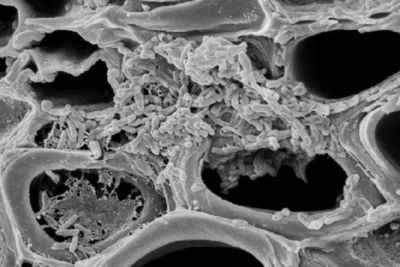
\includegraphics[width=0.32\linewidth, height=!]{img/5}
				\caption{Xylella fastidiosa Temecula1}
			    \label{fig:match5}
			\end{center}
			\end{figure}
	\end{itemize}

	\item \emph{adenosine deaminase} $[$Arcanobacterium haemolyticum DSM 20595$]$~\cite{match6}
	\begin{itemize}
		\item Familia:
		
			Bacteria; Actinobacteria; Actinobacteridae; Actinomycetales;Actinomycineae; Actinomycetaceae; Arcanobacterium.
		\item adenosine deaminase:

			La enzima adenosine deaminase esta relacionada con el metabolismo de las purinas, la ausencia
			de esta produce inmunodeficiencia, y las mutaciones producidas por esta enzima se expresan
			como anemia hemolítica.
		\item Arcanobacterium haemolyticum DSM 20595:

			La bacteria Arcanobacterium haemolyticum es un bacilo grampositivo y es anaerobio facultativo.
			Este microorganismo es causante principalmente de la faringitis y en diabéticos ulceras cutáneas,
			menos común produce meningitis, abscesos, neumonía, entre otras.
		\item Imagen
			\begin{figure}[!h]
			\begin{center}
				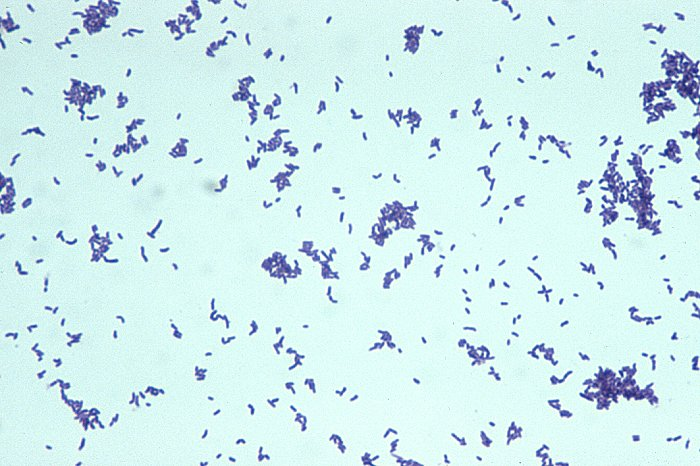
\includegraphics[width=0.32\linewidth, height=!]{img/6}
				\caption{Arcanobacterium haemolyticum}
			    \label{fig:match6}
			\end{center}
			\end{figure}
	\end{itemize}
\end{enumerate}

%% 
Sobre el \textbf{parentesco} de las especies anteriormente señaladas, se obtiene la siguiente información:

Existen 3 grupos de familiares.

\begin{itemize}
	\item El primer grupo está formado por el \textbf{1} y el \textbf{3}, son familiares directo,
		estos gusanos producen la misma enfermedad filariasis cambiando los portadores.
		Sólo difieren en el último elemento de su familia, uno es el Brugia y el otro es el Loa.

	\item El segundo grupo está formado por \textbf{2}, \textbf{4} y nuestro proteína principal 
		\textbf{Agrobaterium tumefaciens}.
		Este grupo esta familiarizado primero las 3 bacterias en la proteobacteria que incluye
		a una gran variedad de patógenos, segundo las dos primeras bacterias están familiarizadas
		hasta la alphaproteobacteria que comprende principalmente géneros fototŕoficos (realizan
		fotosíntesis para obtener energía).

	\item Finalmente existe un elemento aislado de los otros, el número \textbf{5}.
		Este grupo no esta familiarizado con ninguna de las otras bacterias.
\end{itemize}

Cabe destacar que de los 6 microorganismos encontrados existen 2 provenientes de células
eucariotas (Loa y Brugia) y los siguientes 4 de células procariotas (de la primera bacteria encontrada).

%    * Dibuje el "árbol familiar" que muestre las relaciones entre los 6 organismos,
%		de acuerdo a la información en Genbank.
\subsection{Árbol familiar}

Árboles generados a partir de la selección de los 6 primeros matchs y generando el \emph{Distance tree}~\footnote{\url{http://www.ncbi.nlm.nih.gov/blast/treeview/treeView.cgi?request=page&blastRID=AFPY4SHG014&queryID=lcl|21239&distmode=on&entrezLim=&ex=&exl=&exh=&ns=100}}.
\begin{itemize}
%\begin{figure}[h!t]
	\item Rectangle distance tree\\

	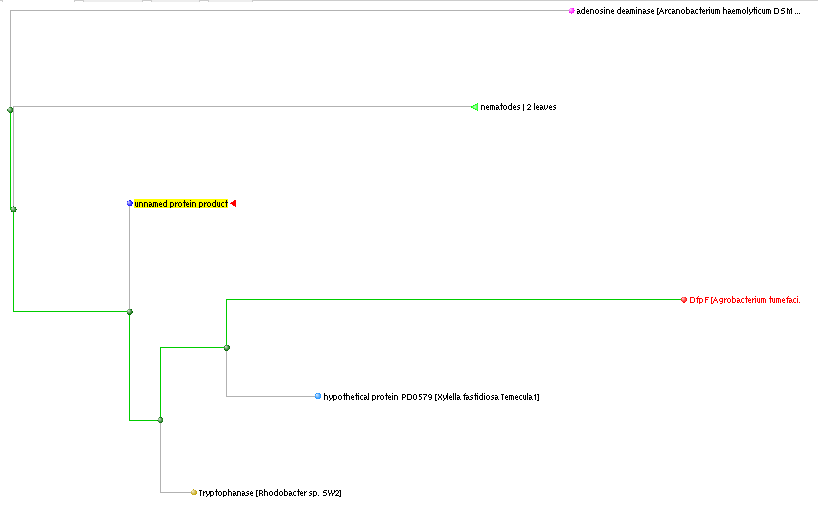
\includegraphics[width=0.8\textwidth]{img/tree_rectangle}
%	\caption{Rectangle distance tree}
%\end{figure}
%
%\begin{figure}[h!t]
	\item Slanted distance tree\\

	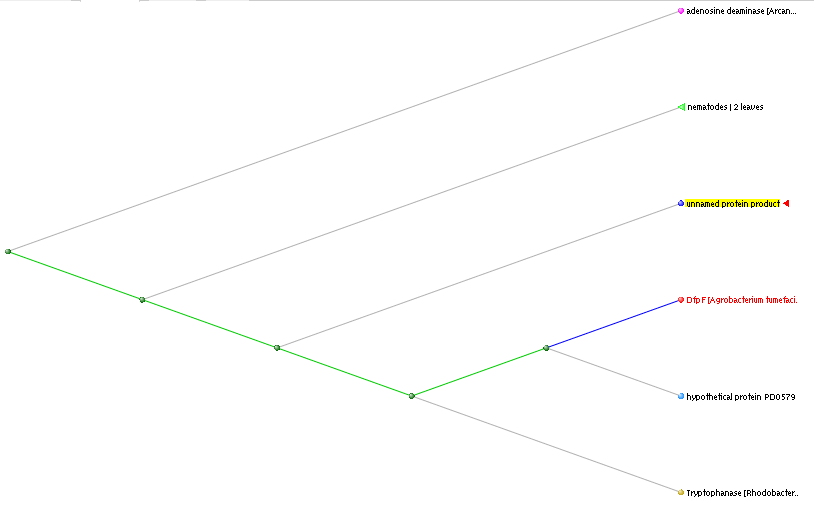
\includegraphics[width=0.8\textwidth]{img/tree_slanted}
%	\caption{Slanted distance tree}
%\end{figure}
%
%\begin{figure}[h!t]
	\item Radial distance tree\\

	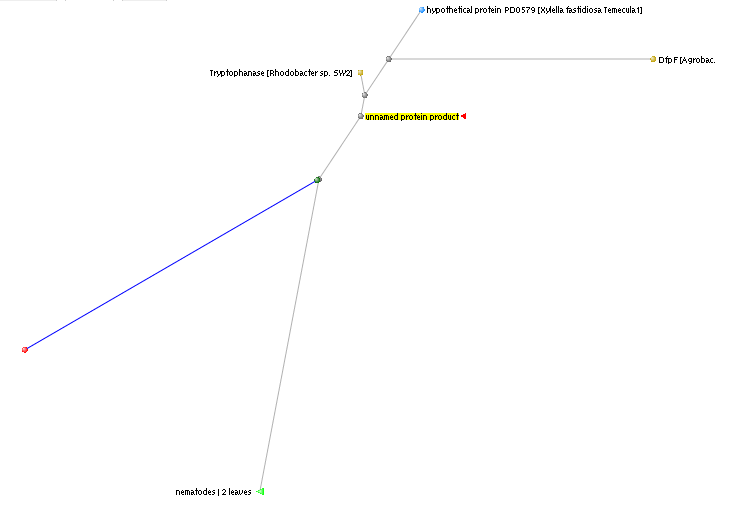
\includegraphics[width=0.8\textwidth]{img/tree_radial}
%	\caption{Radial distance tree}
%\end{figure}
%
%\begin{figure}[h!t]
	\item Force distance tree\\

	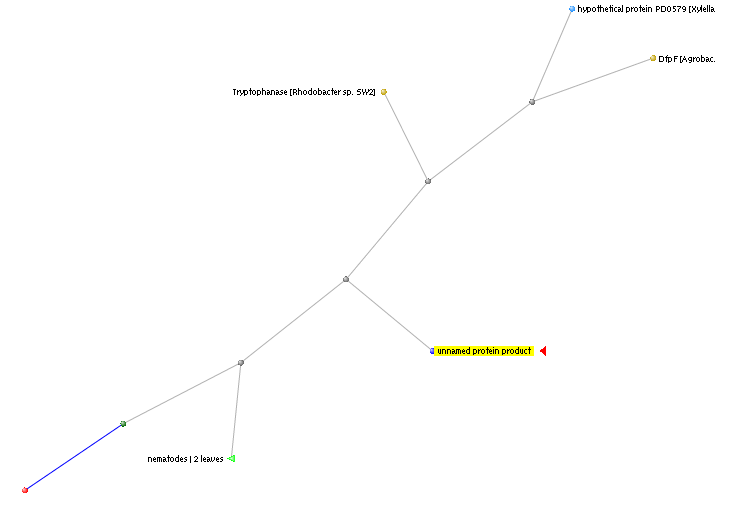
\includegraphics[width=0.8\textwidth]{img/tree_force}
%	\caption{Force distance tree}
%\end{figure}
\end{itemize}
